%--------------------
% Packages
% -------------------
\documentclass[11pt,a4paper]{article}
\usepackage[utf8x]{inputenc}
\usepackage[T1]{fontenc}
%\usepackage{gentium}
\usepackage{mathptmx} % Use Times Font

\usepackage[pdftex]{graphicx} % Required for including pictures
\usepackage[pdftex,linkcolor=black,pdfborder={0 0 0}]{hyperref} % Format links for pdf
\usepackage{calc} % To reset the counter in the document after title page
\usepackage{enumitem} % Includes lists

\frenchspacing % No double spacing between sentences
\linespread{1} % Set linespace
\usepackage[a4paper, lmargin=0.1666\paperwidth, rmargin=0.1666\paperwidth, tmargin=0.1111\paperheight, bmargin=0.1111\paperheight]{geometry} %margins
%\usepackage{parskip}
\usepackage{pdfpages}

\usepackage[all]{nowidow} % Tries to remove widows
\usepackage[protrusion=true,expansion=true]{microtype} % Improves typography, load after fontpackage is selected

\usepackage{listings}
\usepackage{xcolor}

\definecolor{cmdbackground}{RGB}{245,247,249}
\definecolor{cmdborder}{RGB}{180,185,190}
\definecolor{cmdtext}{RGB}{35,39,42}

\lstdefinestyle{commandprompt}{
    basicstyle=\ttfamily\small\color{cmdtext},
    backgroundcolor=\color{cmdbackground},
    frame=single,
    rulecolor=\color{cmdborder},
    framesep=6pt,
    xleftmargin=8pt,
    xrightmargin=8pt,
    framexleftmargin=6pt,
    framexrightmargin=6pt,
    breaklines=true,
    columns=fullflexible,
    keepspaces=true,
    showstringspaces=false,
    aboveskip=10pt,
    belowskip=10pt
}

%-----------------------
% Set pdf information and add title, fill in the fields
%-----------------------
\hypersetup{ 	
pdfsubject = {},
pdftitle = {},
pdfauthor = {}
}

%-----------------------
% Begin document
%-----------------------
\begin{document}
\section*{Submitted by: Hillson Ghimire}
\section*{Task 1: Anaconda Information}

\begin{lstlisting}[style=commandprompt, title={\textbf{Command Prompt: \texttt{conda info}}}]
     active environment : base
    active env location : C:\Users\ghimi\anaconda3
            shell level : 1
       user config file : C:\Users\ghimi\.condarc
 populated config files : C:\Users\ghimi\anaconda3\.condarc
                          C:\Users\ghimi\anaconda3\condarc.d\anaconda-auth.yml
          conda version : 26.5.3
    conda-build version : 26.5.0
         python version : 3.14.6.final.0
                 solver : libmamba (default)
       virtual packages : __archspec=1=skylake
                          __conda=26.5.3=0
                          __win=10.0.26200=0
       base environment : C:\Users\ghimi\anaconda3  (writable)
      conda av data dir : C:\Users\ghimi\anaconda3\etc\conda
  conda av metadata url : None
           channel URLs : https://repo.anaconda.com/pkgs/main/win-64
                          https://repo.anaconda.com/pkgs/main/noarch
                          https://repo.anaconda.com/pkgs/r/win-64
                          https://repo.anaconda.com/pkgs/r/noarch
                          https://repo.anaconda.com/pkgs/msys2/win-64
                          https://repo.anaconda.com/pkgs/msys2/noarch
          package cache : C:\Users\ghimi\anaconda3\pkgs
                          C:\Users\ghimi\.conda\pkgs
                          C:\Users\ghimi\AppData\Local\conda\conda\pkgs
       envs directories : C:\Users\ghimi\anaconda3\envs
                          C:\Users\ghimi\.conda\envs
                          C:\Users\ghimi\AppData\Local\conda\conda\envs
    temporary directory : C:\Users\ghimi\AppData\Local\Temp
               platform : win-64
             user-agent : conda/26.5.3 requests/2.34.2 CPython/3.14.6 Windows/11 Windows/10.0.26200 solver/libmamba conda-libmamba-solver/26.7.0 libmambapy/2.3.2 aau/0.8.1 c/. s/. e/.
          administrator : False
             netrc file : None
           offline mode : False
\end{lstlisting}

\section*{Task 2: Numpy Operations}

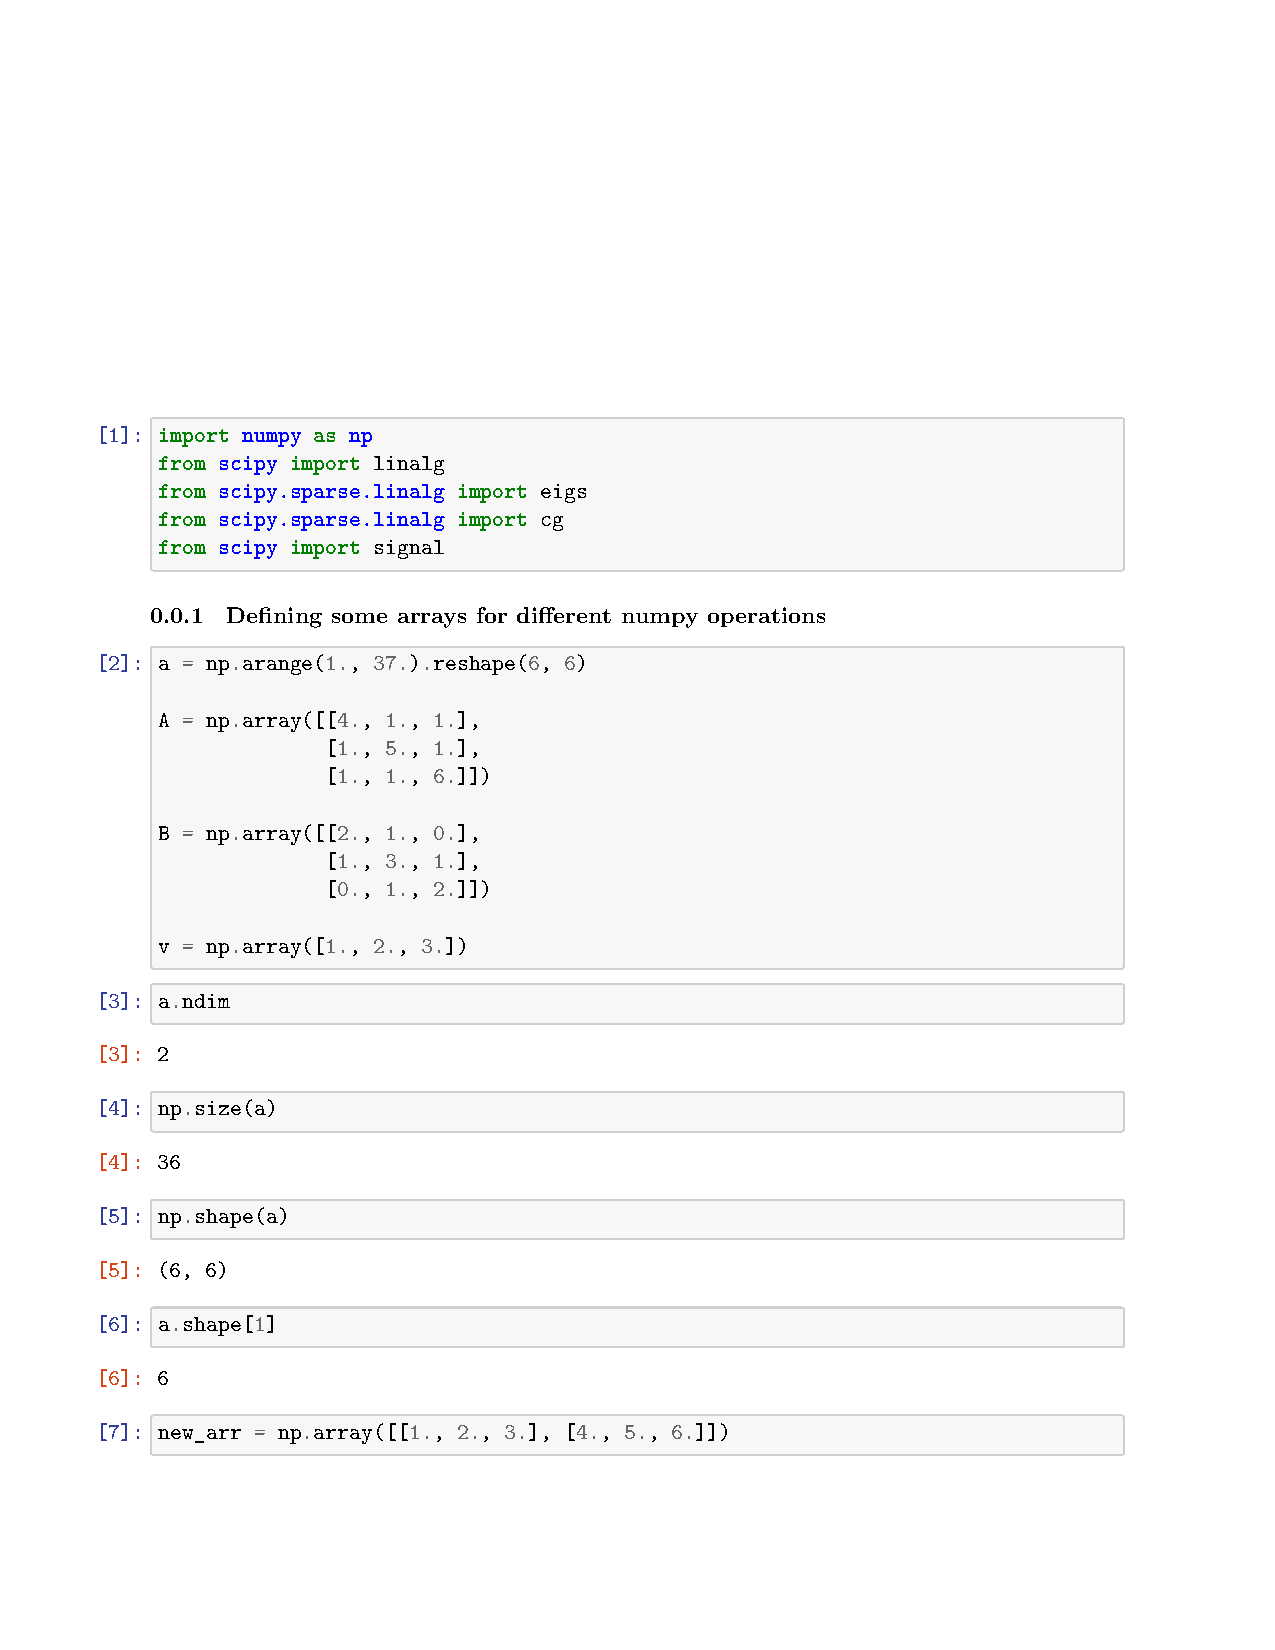
\includepdf[
    pages=1-14, pagecommand={\thispagestyle{plain}}]{numpy_new.pdf}

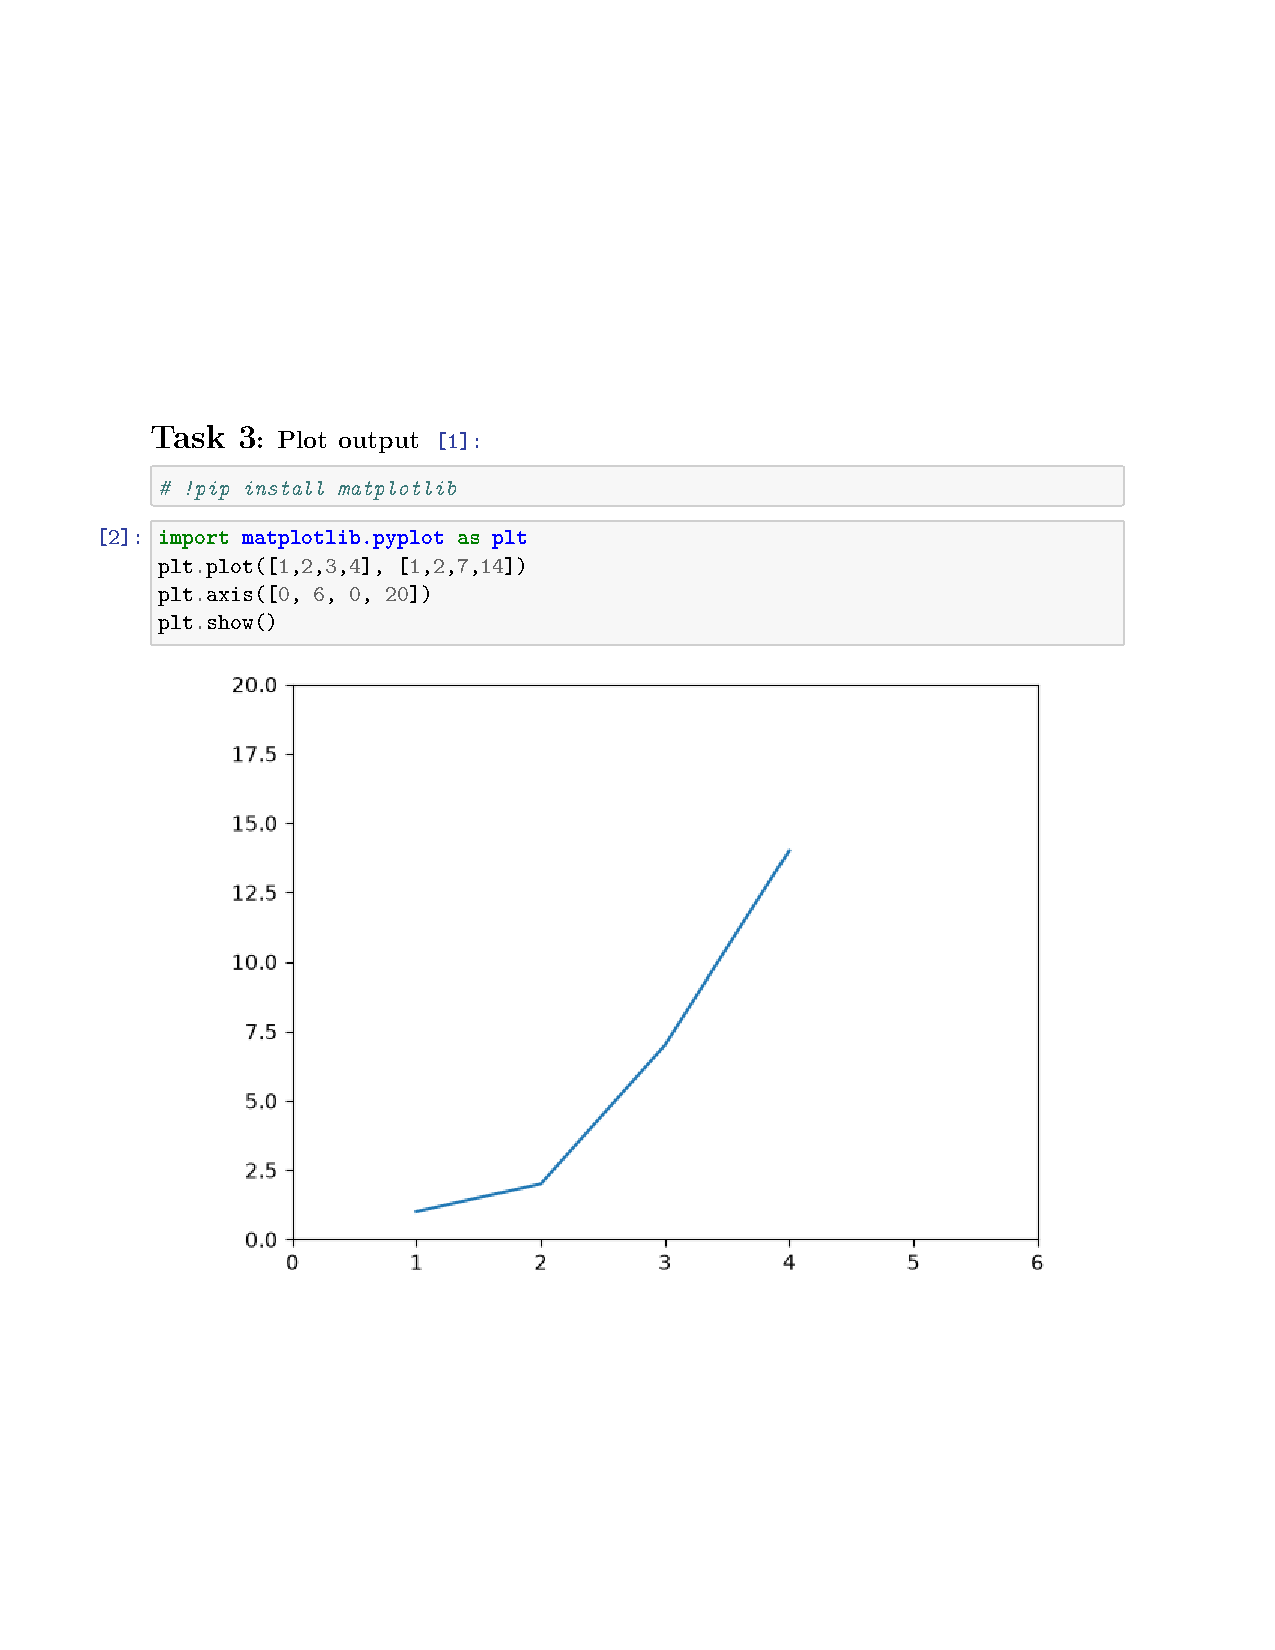
\includepdf[pages=1-2, pagecommand={\thispagestyle{plain}}]{task3.pdf}

% \section{Introduction}
% Test Paragraph


% \subsection*{Subtitle}
% Test Paragraph
\end{document}
